% ACL 2023 proceedings format.
% Drop this file, custom.bib and figures/ into the Overleaf template at
% https://www.overleaf.com/latex/templates/acl-2023-proceedings-template/qjdgcrdwcnwp
% The \IfFileExists below picks up whichever style file that template ships.
\documentclass[11pt]{article}

\IfFileExists{acl2023.sty}{\usepackage{acl2023}}{\usepackage{acl}}

\usepackage{times}
\usepackage{latexsym}
\usepackage[T1]{fontenc}
\usepackage[utf8]{inputenc}
\usepackage{microtype}
\usepackage{graphicx}
\usepackage{booktabs}
\usepackage{amsmath}
\usepackage{amssymb}

\title{Frequency or Information? A Controlled Study of Spectral\\Side-Channel Conditioning in Graph Diffusion}

\author{
  Tamara Bluzer \quad Dan Shamia \quad Daniel Halperin \quad Itamar Kolodny \\
  \texttt{315287441} \quad \texttt{208004119} \quad \texttt{207826314} \quad \texttt{211490362} \\
  Tel Aviv University
}

\begin{document}
\maketitle

\begin{abstract}
Spectral conditioning is standard in graph generation, but in existing generators the truncated
spectrum \emph{is} the representation being generated, which ties ``which frequency band helps''
to ``how much of the graph that representation already carries.'' We separate the two: we diffuse
the full adjacency matrix and supply the truncated normalized-Laplacian spectrum only as a
\emph{side channel}, so band and cutoff $k$ are the only quantities that vary, and we add a model-free probe measuring how much of the target each condition gives away. On SPECTRE's Planar benchmark, five conditioning arms over five cutoffs show no
frequency gradient: 23 of 25 cells sit within one standard deviation of the unconditioned
baseline, and the effect is confined to two isolated minima that the probe separates. Low-frequency conditioning at $k{=}8$
improves the MMD Ratio $2.3\times$ while recovering $0.0\%$ of the target's edges; high-frequency
conditioning at $k{=}32$ improves it $29.7\times$ but recovers $98.5\%$, a near-oracle
regime rather than a frequency effect.
\end{abstract}

\section{Introduction}
\label{sec:intro}

Topology-only graph generation learns a distribution over adjacency matrices with no node or edge
features, so connectivity is the only thing modelled. Diffusion models now
dominate the area \citep{niu2020edpgnn,jo2022gdss,vignac2023digress}, and a recurring idea is to
hand the generator the graph's Laplacian spectrum. \citet{martinkus2022spectre} generate
eigenpairs with a GAN and decode an adjacency matrix from them; \citet{minello2025ggsd} diffuse
the spectrum itself; \citet{vignac2023digress} feed Laplacian eigenfeatures to their denoiser as
fixed extra inputs; and \citet{zhu2025sdmg} argue, for representation learning, that the
low-frequency part of the spectrum carries the useful global information.

These motivate an obvious question --- \emph{which} part of the spectrum helps generation? ---
that existing designs cannot answer cleanly. When the truncated spectrum $(\lambda_k,
U_k)$ is the representation the model generates and decodes from, $k$ controls the frequency
content of the condition \emph{and} how much of the target that representation
determines. On $n{=}64$ planar graphs $U_k \mathrm{diag}(\lambda_k) U_k^\top$ at $k{=}32$ is close
to the Laplacian itself, so a band that ``wins'' there may simply be inverting its own condition.
No cited work reports a condition-information floor against which its frequency curve could be
read.

\paragraph{Research question.} \emph{Given a diffusion model whose state already carries the full
graph, does an explicit spectral side channel improve generation, and does the incremental benefit
depend on which frequency band and how many eigenpairs are supplied?}

Phrasing it as a side channel makes the question falsifiable. Every arm diffuses the same object
with the same architecture and budget and receives a condition tensor of the same shape; only the
\emph{selection} of eigenpairs differs. A \texttt{none} arm gives the null, and three controls ---
a random band, shape-matched Gaussian noise, and another graph's real low band --- separate
frequency-specific information from conditioning capacity and from generic spectral statistics. We
then add the measurement the literature lacks: a model-free probe that reconstructs edges
from the condition alone.\footnote{Code and run artifacts:
\url{https://github.com/TamaraBluzer/Frequency_aware_diffusion-}.
\texttt{scripts/make\_paper\_figures.py} rebuilds both figures from \texttt{results/*.json} with
no hand-typed number.}

Our contributions are that design; the central negative result that there is \textbf{no frequency
gradient} (\S\ref{sec:sweep}); a leakage probe that \textbf{separates the two minima}
(\S\ref{sec:leakage}), showing the study's strongest number to be a near-oracle regime rather than
a frequency effect; a diagnosis of the universal $0\%$ validity (\S\ref{sec:validity}); and two
further negative results (\S\S\ref{sec:e2e}--\ref{sec:downstream}).

\section{Related Work}
\label{sec:related}

\paragraph{SPECTRE} \citep{martinkus2022spectre} is the closest methodological and evaluation
reference: a GAN generates $(\lambda_k, U_k)$ on a Stiefel manifold, then a graph network builds
the adjacency matrix from $U_k \mathrm{diag}(\lambda_k) U_k^\top$. It sweeps $k \in \{2,4,8,16,32\}$ on Planar and SBM --- the grid we reuse --- but picks
one $k$ per dataset heuristically and never reports the curve. We treat $k$ and the band as the object of
study, replace its sign-canonicalization heuristic with a sign- and basis-invariant pair channel,
and diffuse adjacency rather than decoding a generated spectrum.

\paragraph{GGSD} \citep{minello2025ggsd} already measures smallest- versus largest-eigenpair
representations inside a diffusion generator, so frequency-band sensitivity is not itself novel.
Ours is narrower: the incremental value of a side channel while the diffusion state
still carries the full graph, with matched-capacity controls and a measured information floor.

\paragraph{Others.} \textbf{DiGress} \citep{vignac2023digress} supplies our datasets, discrete
process and evaluation suite, and feeds Laplacian eigenvalues to its denoiser as a fixed
augmentation rather than a variable to ablate --- exactly the variable we isolate. \textbf{LGD}
\citep{zhou2024lgd} runs latent diffusion on molecules under scalar property conditioning;
\S\ref{sec:model} says why we abandoned its design. \textbf{DualDiff} \citep{xie2026dualdiff}
couples node- and cluster-level latents, but a cluster count collapses global structure into one
number, where an eigenpair-indexed condition exposes an ordered band and so admits a sweep.
\textbf{SDMG} \citep{zhu2025sdmg} finds low-frequency reconstruction beating full-spectrum
reconstruction for \emph{representation} learning; we ask whether that transfers to
\emph{generation}.

\section{Method}
\label{sec:method}

\paragraph{Data.} SPECTRE's released Planar benchmark: 200 graphs at $n{=}64$, each a Delaunay
triangulation of uniform random points, split 128/32/40 following DiGress's recipe, which we re-process ourselves since its
\texttt{process()} appends every graph twice. Each arm generates 32 graphs, matching the
evaluation set.
\textbf{Every number here is scored on the validation split}, which also selected the checkpoints
(since lost), so all results are optimistic in the usual way.

\paragraph{Spectral condition.} Let $L = I - D^{-1/2} A D^{-1/2} = U \Lambda U^\top$ with $0 =
\lambda_1 \le \dots \le \lambda_n \le 2$, and let $t$ be the number of zero eigenvalues
(equivalently, connected components). The arms take $k$ eigenpairs as \texttt{low} $=
(\lambda_{t+1} \dots \lambda_{t+k})$, \texttt{high} $= (\lambda_{n-k+1} \dots \lambda_n)$,
\texttt{random} $=$ $k$ indices drawn uniformly from $t{+}1 \dots n$, \texttt{gaussian} $=$
i.i.d.\ $\mathcal{N}(0,1)$ tensors of identical shape, \texttt{shuffled} $=$ another graph's real
low band under a derangement, and \texttt{none} $=$ an all-zero condition with a presence flag.

The condition enters the denoiser twice: as a pair channel $\big(U_k \mathrm{diag}(\lambda_k)
U_k^\top\big)_{ij}$, rescaled per graph to unit RMS so \texttt{low} and \texttt{high} cannot differ in activation
scale, and as the selected eigenvalues mapped from $[0,2]$ to $[-1,1]$, supplied globally with the
timestep. The pair channel is invariant to eigenvector sign flips
and to rotations within an exactly repeated eigenspace, sidestepping the ambiguity that motivates
SignNet \citep{lim2023signnet} without depending on it.

\paragraph{Model.}
\label{sec:model}
The diffusion state is the centred adjacency matrix $x_0 = 2A - 1$. A cosine forward process
\citep{nichol2021improved} adds symmetric Gaussian noise to each undirected pair, and a permutation-equivariant DiGress transformer predicts $x_0$ from $x_t$
\citep{ho2020ddpm,vignac2023digress}, masking the diagonal and padding at every step. It has
4 layers ($d_x{=}128$, $d_e{=}64$, $d_y{=}128$, 8 heads; 1.83M parameters), $T{=}100$ steps, and
trains 200 epochs at batch 16, learning rate $3\!\times\!10^{-4}$, with the condition dropped at
probability $0.1$ to enable guidance at sampling time \citep{ho2022cfg}. We began from an LGD-style autoencoder and abandoned it after measuring it: its per-pair latent is
an expansion, not a compression (32{,}768 floats for 2{,}016 binary decisions), and reaches F1
$=1.000$ only by copying $A_{ij}$ down a private lane.

\paragraph{Evaluation.} We reimplement the GraphRNN/GRAN/SPECTRE suite
\citep{you2018graphrnn,liao2019gran,martinkus2022spectre}: MMD \citep{gretton2012mmd} under a
total-variation Gaussian kernel over degree histograms, clustering coefficients,
normalized-Laplacian eigenvalues, 12 ab-spline wavelet scales, and 4-node orbit counts via ORCA
\citep{hocevar2014orca}. Raw MMD is uninterpretable, so we report \textbf{Ratio}: each metric
divided by its train-vs-test floor and averaged, so $1.0$ means indistinguishable from real data
at this sample size. Validity is \texttt{networkx} planarity \emph{and} connectivity \citep{hagberg2008networkx}. We calibrated the harness before
training any model of ours: real-vs-real scores ${\approx}0$, the floor is $1.00$ by construction,
and a \emph{per-graph density-matched} Erd\H{o}s--R\'enyi control \citep{erdos1959random} scores
$3035\times$ it.

\paragraph{Protocol and leakage probe.} Each arm uses three seeds at equal compute; band
comparisons use a paired hierarchical bootstrap (1{,}000 resamples) over graphs and seeds. The
\textbf{leakage probe} is model-free: it scores every node pair by $\big(U_k
\mathrm{diag}(\lambda_k) U_k^\top\big)_{ij}$ --- exactly the tensor the denoiser receives --- and
keeps the $m$ highest-scoring pairs, where $m$ is the target's true edge count. Using the true edge and node counts is deliberately privileged: the probe upper-bounds what any
decoder could extract, so a low score is strong evidence a band cannot leak. Gaussian conditions score at chance, and the full spectrum recovers $100.0\%$, as it must.

\section{Results}
\label{sec:results}

\paragraph{Three run families.}
\label{sec:runfamilies}
Results below come from three run sets at identical architecture and budget: the $k{=}8$
\emph{pilot} (Table~\ref{tab:k8}), the \emph{sweep} (Figure~\ref{fig:sweep}, seed 0 only), and the
\emph{seed confirmation} of the two minima (Table~\ref{tab:spikes}). Each therefore estimates the
same unconditioned baseline --- $327.2$, $335.7$, $330.1$, agreeing to within one seed standard
deviation --- and \texttt{low} $k{=}8$ appears as $158.0$, $116.3$ and $141.9$, a spread
consistent with that arm's own $\pm19.3$ across seeds. Every comparison below is \emph{within} one
set, against that set's own baseline.

\subsection{Conditioning helps at $k{=}8$}
Table~\ref{tab:k8} is the kill gate we set before anything downstream. Low-frequency conditioning
halves the Ratio and cuts validation loss by 60\%, while high and random conditioning are
indistinguishable from \texttt{none}. Paired bootstrap 95\% intervals for
\texttt{low} minus \texttt{none}, \texttt{high} and \texttt{random} are $[-189.4, -152.1]$,
$[-206.7, -152.4]$ and $[-195.1, -142.2]$, all excluding zero by a wide margin. The model
demonstrably uses the condition: under identical diffusion noise, adding it changes $12.95\%$ of
edge decisions. Figure~\ref{fig:samples} shows the gap. All arms match the target density and none
is planar in any of its 32 samples, so validity cannot separate them; triangle count can. Against
a real graph's $118$, \texttt{low} manages $116$ where \texttt{none}, \texttt{high} and
\texttt{random} manage $15$, $15$ and $13$: what the low band supplies is the local mesh a
triangulation is made of.

\begin{table}[t]
\centering\footnotesize
\setlength{\tabcolsep}{4pt}
\begin{tabular}{lccc}
\toprule
band & Ratio $\downarrow$ & val.\ loss $\downarrow$ & valid \\
\midrule
\texttt{none}   & 327.2 $\pm$ 8.8  & 0.132 $\pm$ 0.012 & 0\% \\
\texttt{low}    & \textbf{158.0 $\pm$ 16.2} & \textbf{0.053 $\pm$ 0.004} & 0\% \\
\texttt{high}   & 339.1 $\pm$ 9.2  & 0.094 $\pm$ 0.009 & 0\% \\
\texttt{random} & 326.5 $\pm$ 11.8 & 0.128 $\pm$ 0.012 & 0\% \\
\bottomrule
\end{tabular}
\caption{Oracle conditioning at $k{=}8$, three seeds, mean $\pm$ std. Validation loss is
metric-free and orders the arms the same way Ratio does. This is the $k{=}8$ pilot, a separate
run family from the sweep of \S\ref{sec:sweep}; \S\ref{sec:runfamilies} reconciles the two.}
\label{tab:k8}
\end{table}

\begin{figure}[t]
\centering
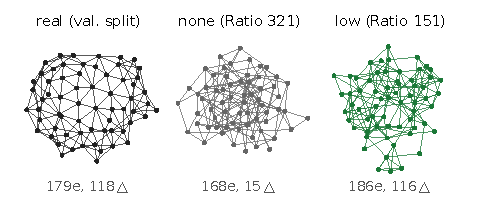
\includegraphics[width=\columnwidth]{figures/samples.pdf}
\caption{Seed-0 samples of two Table~\ref{tab:k8} arms beside a real Planar graph, with edge and
triangle counts. Index $0$ of every arm, not a chosen one, under one shared Kamada--Kawai layout,
so the real graph is \emph{not} handed its triangulation's coordinates. \texttt{high} and
\texttt{random} look like \texttt{none} and are omitted.}
\label{fig:samples}
\end{figure}

\subsection{The sweep: two spikes, not a gradient}
\label{sec:sweep}

\begin{figure*}[t]
\centering

\includegraphics[width=\textwidth]{figures/sweep.pdf}
\caption{Five conditioning arms $\times$ five cutoffs on Planar, seed 0; stars mark three-seed
means $\pm$ std for the two re-run cells. \textbf{(a)} Quality against $k$, baseline dashed.
\textbf{(b)} The same points against measured leakage.}
\label{fig:sweep}
\end{figure*}

SDMG's intuition implies quality should vary smoothly with how much of which end of the spectrum
is supplied. It does not (Figure~\ref{fig:sweep}(a)). Over the 23 conditioned cells that are not one of the two minima, mean Ratio is $327.1 \pm 18.5$,
and the unconditioned baseline of $335.7$ sits $+0.46$ standard deviations \emph{inside} that
spread: the flat region simply is the baseline. Each of those cells is a single seed, so we claim
only that they lie within one standard deviation of the baseline, not that each is individually
tested. Against that spread the minima sit $-10.0$ (\texttt{low}, $k{=}8$, at its three-seed mean)
and $-17.1$ (\texttt{high}, $k{=}32$) standard deviations below, while their neighbours in the
same band show nothing --- on the same seed-0 sweep \texttt{low} is $316.4$ at $k{=}4$ and
$270.5$ at $k{=}16$, against $116.3$ at $k{=}8$.

Both minima reproduce across three seeds (Table~\ref{tab:spikes}): \texttt{high}, $k{=}32$ is very
stable (std $0.58$ on a mean of $11.11$) and the only arm in the sweep that produced a valid
planar graph. \texttt{low}, $k{=}8$ is noisier but never approaches baseline, and its seed-0
draw was its most favourable, so $141.9$ is the number to quote. The controls do
their job: \texttt{gaussian} spans $322$--$333$ and \texttt{shuffled} --- another graph's real low
band --- spans $329$--$342$, both flat on the baseline at every $k$. Neither \emph{having a
condition} nor \emph{having real spectral statistics} suffices; the effect needs the matching
graph's own spectrum at a particular band and cutoff, the cleanest evidence we have that
the mechanism is informational rather than extra capacity.

\begin{table}[t]
\centering\footnotesize
\setlength{\tabcolsep}{5pt}
\begin{tabular}{lccc}
\toprule
arm & Ratio $\downarrow$ & vs.\ base & leak \\
\midrule
\texttt{high} $k${=}32 & \textbf{11.1 $\pm$ 0.6} & 29.7$\times$ & 98.5\% \\
\texttt{low} $k${=}8   & 141.9 $\pm$ 19.3 & 2.3$\times$ & \textbf{0.0\%} \\
\texttt{none}          & 330.1 $\pm$ 6.2 & --- & --- \\
\bottomrule
\end{tabular}
\caption{Three-seed confirmation of the two minima, with edge recovery from the condition alone,
against this family's own \texttt{none} baseline. Both reproduce; only one of them is leak-free.}
\label{tab:spikes}
\end{table}

\subsection{Leakage separates the two minima}
\label{sec:leakage}

\begin{table}[t]
\centering\footnotesize
\setlength{\tabcolsep}{4pt}
\begin{tabular}{lccccc}
\toprule
band & $k${=}2 & $k${=}4 & $k${=}8 & $k${=}16 & $k${=}32 \\
\midrule
\texttt{low}      & 0.0 & 0.0 & \textbf{0.0} & 0.0 & 0.6 \\
\texttt{high}     & 21.8 & 31.4 & 49.3 & 76.7 & \textbf{98.5} \\
\texttt{random}   & 14.8 & 15.6 & 19.2 & 26.3 & 43.6 \\
\texttt{gaussian} & 7.9 & 8.5 & 8.2 & 8.7 & 9.4 \\
\texttt{shuffled} & 8.7 & 8.7 & 8.8 & 8.7 & 8.3 \\
\bottomrule
\end{tabular}
\caption{Edge recovery (\%) from the condition alone, Planar validation split; chance is 8.8\%.
The probe uses the true edge count, so these are upper bounds.}
\label{tab:leakage}
\end{table}

An obvious objection to Table~\ref{tab:k8}: each sample is conditioned on a validation graph's
spectrum and scored against those same graphs, so a band that hands over more of the target wins
for reasons unrelated to frequency. Table~\ref{tab:leakage} measures this, and at
$k{=}8$ the objection is refuted in the strongest possible way: leakage is \emph{anti}-correlated
with quality. \texttt{low} recovers $0.0\%$ of edges --- below chance --- and wins by ${\sim}170$
Ratio points, while \texttt{high} recovers $49.3\%$ and loses. The pattern replicates on SBM (\texttt{low} at or below $3.5\%$ against $9.4\%$ chance,
\texttt{high} $87.7\%$ at $k{=}32$), so it is not an artifact of Planar's construction from 2D
points.

At $k{=}32$, however, leakage and quality \emph{coincide} (Figure~\ref{fig:sweep}(b)): the minima
sit at opposite ends of the information axis and are not the same phenomenon. \texttt{low}, $k{=}8$ improves generation while leaking nothing measurable, so it must
supply coarse global structure the model cannot otherwise infer --- the one genuine frequency
effect here. \texttt{high}, $k{=}32$ supplies a near-complete specification of the target, so it
is closer to handing the model the answer than to selecting a frequency. Reporting its $29.7\times$ improvement without its $98.5\%$ leakage would be misleading ---
exactly the confound the information floor was added to catch.

\subsection{Why validity is zero everywhere}
\label{sec:validity}
Validity is \emph{connected AND planar}, so the universal $0\%$ cannot say which half failed; the
probe's reconstructions separate them.
Connectivity is easy: by $k{=}32$ every reconstruction is connected in both bands, and
\texttt{low} at $k{=}16$ is already $71.9\%$ connected on $0.0\%$ edge recovery. Planarity
essentially never is --- only \texttt{high}, $k{=}32$ reaches it, at $3.1\%$.

That arm explains why. At $98.5\%$ recovery the mean number of misplaced edges is $2.7$ of
${\sim}177$ (max 6), and the fraction with \emph{zero} misplaced edges is $3.1\%$ --- the same $3.1\%$ that is planar,
so every reconstruction with even one wrong edge is non-planar. This is a property of the target
class, not our model: a planar graph on $n{=}64$ with 177
edges sits near the $3n-6 = 186$ bound, so it is nearly maximally triangulated and almost any
added chord creates a $K_5$ or $K_{3,3}$ minor. Validity is therefore close to a binary test of
exactness, not a graded measure, which is why an arm can improve Ratio $2.3\times$
while pinned at zero. The usual prescription --- add structural features --- has negative
precedent in our own runs: the discrete arm of \S\ref{sec:e2e} includes cycle counts and still
reports $0\%$ validity at every scale.

\subsection{From oracle to end-to-end}
\label{sec:e2e}
Everything above is oracle-conditioned: the spectra come from held-out real graphs, so these
arms are a diagnostic upper bound rather than a generative model. To close it we trained a diffusion prior over $(n, \lambda_k, U_k)$ with an orthogonality penalty
and a QR retraction at the final step, then sampled end to end. Against an ER reference of $161.67$,
oracle spectra give Ratio $5.92$ (\texttt{high}, $k{=}32$) and $74.86$ (\texttt{low}, $k{=}8$);
end to end at guidance scale 1 these become $159.72$ and $295.64$, so the low arm fails its gate
outright. Guidance is U-shaped over $\{0.5,1,1.5,2,3\}$, optimal at $1.5$, and even there a
$24\times$ degradation remains, because small eigenvector errors compound through $U
\mathrm{diag}(\lambda) U^\top$. These Ratios omit ORCA and are
\emph{not} comparable to the tables above, hence the ER reference.

A discrete-diffusion arm \citep{austin2021d3pm} sharpens the caveat. At a serious budget (10
layers, 500 steps, 1{,}000 epochs) the \emph{unconditioned} baseline improves ${\sim}8\times$, from ${\sim}327$ to
$39.60$; conditioning still helps, to $15.40$ ($-61\%$), but the gap narrows from ${\sim}220$
Ratio points to ${\sim}24$. A small-budget headline overstates conditioning's contribution, and validity stays $0\%$ at
every scale.

\subsection{Downstream utility: a negative result}
\label{sec:downstream}
The intended payoff is synthetic augmentation. We test it on a task
deliberately aligned with the hypothesis --- predicting an SBM graph's community count (2--5),
which is what low-frequency eigenvalues encode --- with 20/40/80 real training graphs and 5 seeds,
each augmented graph conditioned on a real training graph and inheriting its label. Diffusion augmentation never beats real-only training: at $n{=}20$
unconditioned augmentation hurts ($89.8\%$ against $94.8\%$) and conditioned
augmentation is no better ($92.0\%$); at $n{=}80$ both stay below the $97.2\%$ baseline. Fresh
samples from the \emph{true} SBM generator do help slightly ($98.8\%$ at $n{=}80$), locating the
failure in sample quality rather than the pipeline. The task is also easy to begin with, so this shows the gains of \S\ref{sec:sweep}
do not automatically become downstream utility, not that they never could.

\section{Discussion and Conclusion}
\label{sec:discussion}

\paragraph{What the side channel buys.} Very little, almost everywhere: given a diffusion state that already carries the full graph, a
truncated spectrum is worthless in 23 of 25 configurations, and the two exceptions differ in kind. The real finding is \texttt{low}, $k{=}8$ --- a $2.3\times$ Ratio improvement and 60\% lower
validation loss from a condition a privileged probe cannot use to recover one edge above chance,
hard to explain as anything but coarse global structure that is useful and hard to infer alone.
\texttt{high}, $k{=}32$ is the better number and the weaker result: without the probe we would
have reported a near-oracle regime as our headline. That a controlled study can invert its own
top-line claim is our best argument for an information floor none of the cited work reports.

\paragraph{Two caveats on our own reporting.} First, the sharpness is unexplained: both minima reproduce ten to seventeen standard deviations
below a flat surface, so they are real, but no mechanism predicts \emph{which} cells spike.
Second, Ratio averages whichever metrics were available, and orbit's tiny
floor dominates any mean it enters: seed-0 \texttt{none} is $321.21$ with ORCA and $125.25$
without, a $2.56\times$ gap that brackets the unexplained $2.09\times$ ER reference shift
($337.91$ vs.\ $161.67$). Orbit contributes $84.0\%$ of the $k{=}8$ improvement while \emph{degree
moves the wrong way}, and a geometric mean puts the aggregate at $-34.8\%$ rather than $-52.9\%$.
The low-band result survives --- it wins on four of five metrics and on validation loss --- but
the arithmetic mean overstates it.

\paragraph{Limitations.} (i) Every number is validation-split, on splits that also selected
checkpoints, and validity is $0\%$ throughout, so we compare distributional fidelity, not sample
correctness. (ii) The quality sweep is Planar only --- on SBM we ran the leakage half, which
replicates, not the generation half --- and SBM validity uses a spectral-clustering stand-in.
(iii) The sweep's values come from a recycled Colab stdout, so its per-metric
breakdowns are lost; ORCA was verified present, so they are five-metric. (iv) Our
discrete model is not a DiGress reproduction, and four planned ablations were not run.

\bibliographystyle{acl_natbib}
\bibliography{custom}

\end{document}
